\section{Now Forecasting Methodology} %3.5

\subsection{K-Fold Cross-validation}
\begin{figure}[htbp]
    \center
    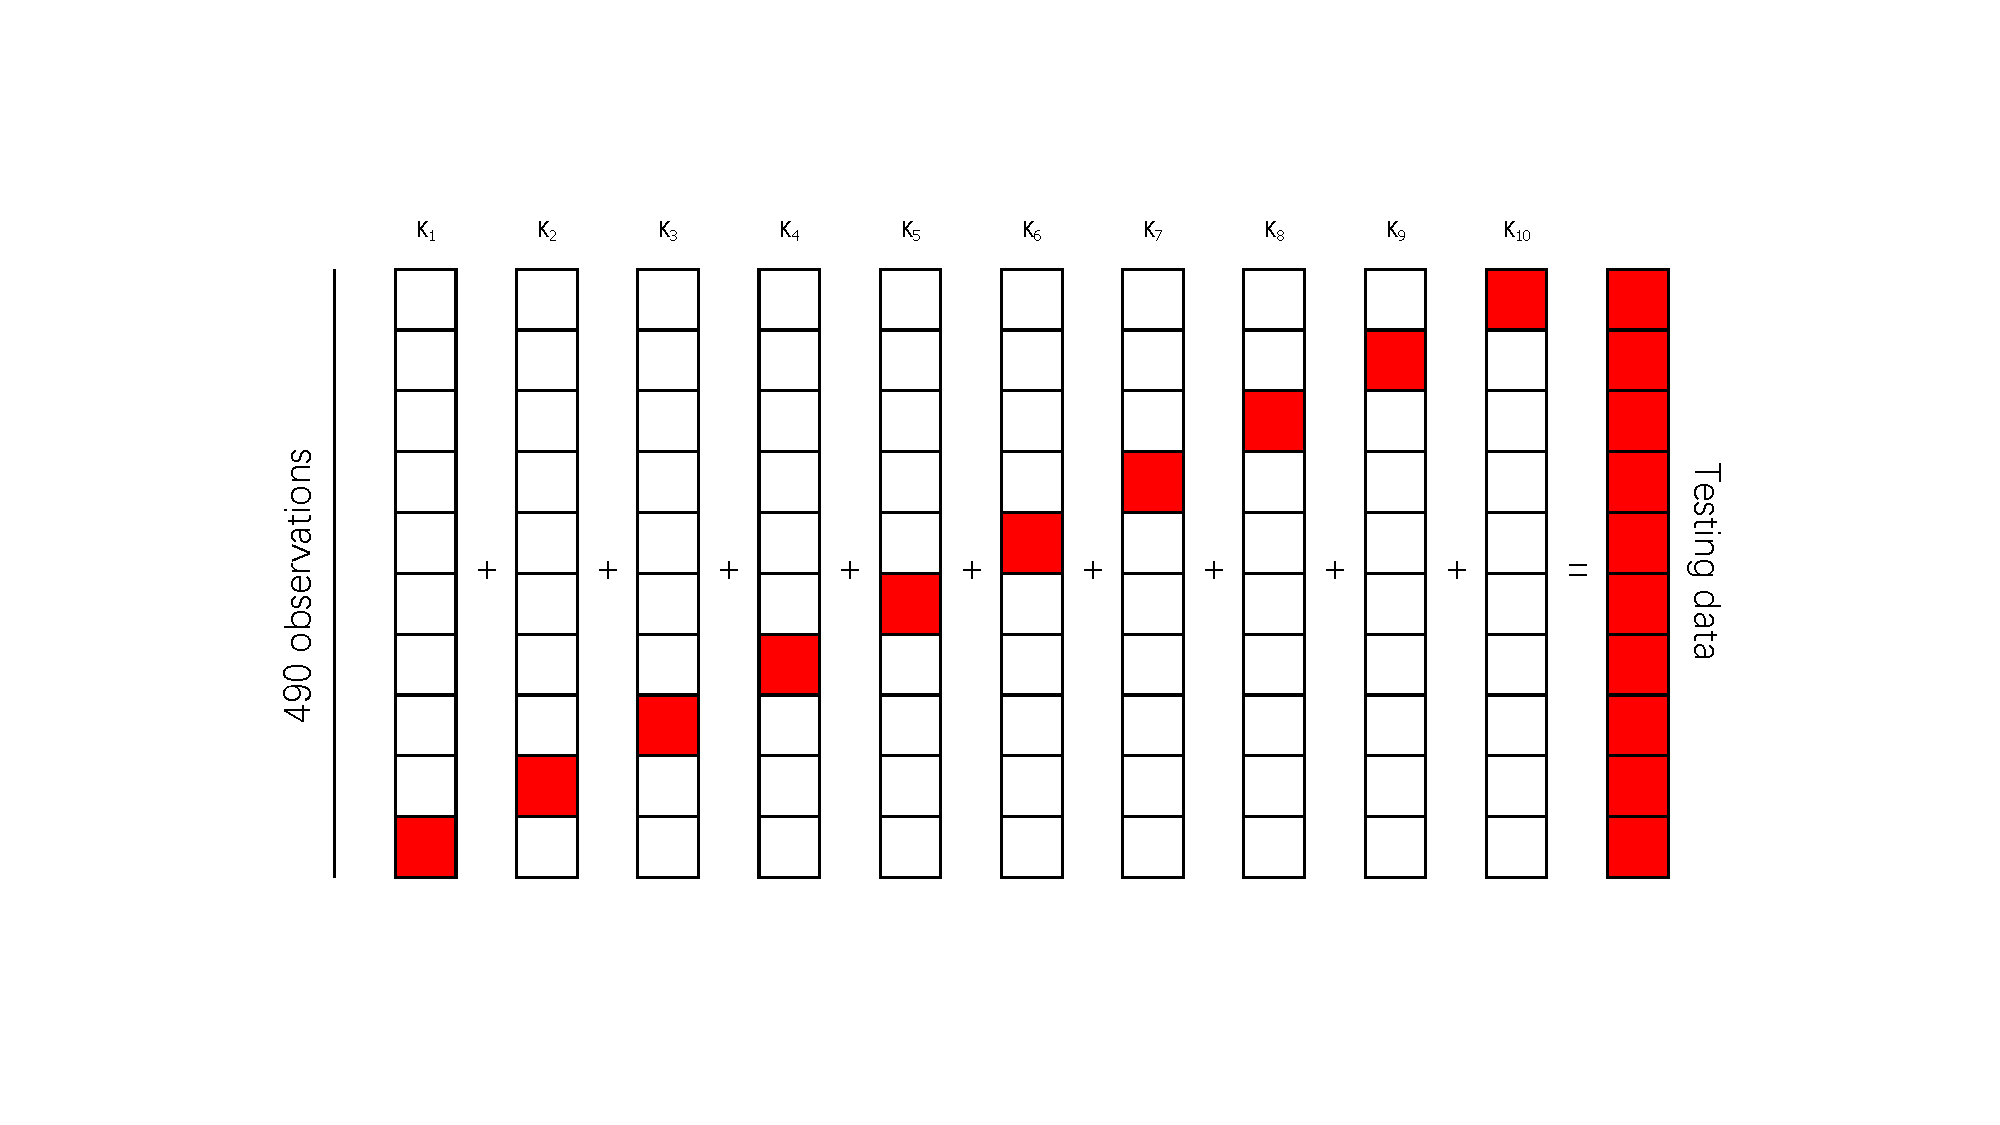
\includegraphics[scale=0.4]{Figure/3.5.1-K-Fold.pdf}
    \caption{K-fold Cross-validation}
    \label{3.5.1-K-Fold}
\end{figure}

Cross-validation is a data splitting and testing method. In this project, k-fold splits the data set into 10 parts. Each time, 9 parts represented by the white grid in Figure \ref{3.5.1-K-Fold} are used as training data, and the remaining part represented by the red grid in Figure \ref{3.5.1-K-Fold} is used as testing data for model validation. Since k-fold cross-validation is suitable for small data scenarios, it was applied in this project where only 490 observations are contained in the data set.


\subsection{Linear Regression}
Linear regression uses statistical analysis to determine the quantitative relationships between multiple variables \cite{montgomery2012introduction}. By a given training set, one reasonable method to pick or learn the parameters $\theta$ is to make the hypothesis $h(x)$ close to $y$. To formalize this, we will define a function that measures, for each value of the $\theta$'s, how close the $h (x^{(i)})$'s are to the corresponding $y^{(i)}$'s. We define the cost function or ordinary least squares:

\begin{eqnarray}
    J_\theta = \frac{1}{2} \sum_{i=1}^{n}{(h_\theta (x^{(i)}) - y^{(i)})^2}.
    \label{eq:cf}
\end{eqnarray}

After minimising the sum of the residual, the weights vector for each independent variable will be generated. In the result, P-value of each feature is also notable and can be applied to express the magnitude of the significant influence of the independent variable on the dependent variable. However, owing to the low deviation of linear regression, as the number of features increases, it is susceptible to high variance or over-fitting.

\subsection{Penalised Linear Regression (Lasso, min/1se)}
Comparing with linear regression, Penalised regression is a highly computationally efficient prediction method that can reduce a large number of features into a manageable set and make good predictions on various large data sets, especially when the features are correlated.\cite{bowles2015machine}. As Function \ref{eq:new-cf} shown, a penalty term with coefficient Lambda is added to cost function to penalise model complexity by limiting the weight magnitude for reducing the variance.

\begin{eqnarray}
    J_\theta := J_\theta + \lambda \sum_{K=1}^{k}{b_k}.
    \label{eq:new-cf}
\end{eqnarray}

In the project, Lasso regression was applied. Comparing with ridge regression, which is also a form of Penalised Regression, Lasso regression is able to cancel unimportant features based on the choice of Lambda. Generally, the choice of Lambda is based on the MSE. In this algorithm, the k-fold method was applied for calculating MSE with a different value of Lambda. 

Based on MSE, there are two methods to choose coefficient Lambda which are \sys{min} and \sys{1se}. These two methods have different preferences. Applying \sys{min} is intended to obtain the model with the minimum error and the most accurate, while \sys{1se} tends to simplify the model as much as possible with the loss of a small amount of accuracy.

\subsection{Penalised Polynomial Regression (Lasso, min/1se)}
For linear regression and penalised linear regression, due to the lack of flexibility, the fitting result is often poor. Facing this problem, features with higher-order were applied in them for training. Similarly, when the features of higher-order were added to the model for raising flexibility, the polynomial regression may also have the problem of over-fitting. Therefore, similar to linear regression, Lasso penalisation was also added, simplifying models while addressing the problem of over-fitting.

\subsection{Random Forest}
Random Forest is a model that uses the main vote of multiple decision trees to achieve prediction. It can be applied both on regression and classification algorithm \cite{tan2018prediction}. For Random Forest, $n$ training samples with $i$ features (less than the total number of features) are randomly selected from the original data sets using Bootstrapping method that is a type of reaping sampling method. After $k$ rounds of random selection, $k$ independent training sets are selected and $k$ decision trees are generated.

Due to the randomness of observation selection, non-selected observations are defined as out-of-bag data. Use these observations as labelled testing data, out-of-bag errors (\sys{OOB}) can be calculated. As  $k$ increases, \sys{OOB} will decrease and tend to be stable. Selecting the appropriate k value based on the \sys{OOB} is critical.  Small $k$ value causes \sys{OBB} instability  while great $k$ value brings high Computational cost.

Also, the feature number applied in each decision tree $i$ can be also important. Small $i$ value causes low flexibility problem, while great $i$ value reduce the diversity of the "forest". Generally, with the increase of $i$, \sys{OOB} value drops first and then rises. Choosing the $i$ value corresponding to the minimum \sys{OBB} helps to achieve better performance of the model.

\subsection{Neural Networks}
A neural network is a massively parallel processor composed of simple processing units. Neurons are formed the basic structure of the network. With the structure of multiple hidden layers, Neural networks algorithm is highly flexible for fitting but also suffers from over-fitting and high computational cost problem. 

Forward propagation is a process that multiple inputs enter a hidden layer and time corresponding weights. After that, a nonlinear activation function is applied to convert the input signal into an output signal. For training Neural Networks, backpropagation method is applied. Through gradient descent of loss function, the weights in the whole network can be updated. Since the application of differential operation, the computational cost of training can be mainly attributed to backpropagation.






